\section{\esp Introdução}
Com a mudança de mentalidade da Web 1.0 para o novo paradgma de aplicações web conhecido como Web 2.0 proposta por \cite{web20Proposta}, seus 
usuários deixaram de ter um papel passivo como consumidores de conteúdo para assumir um papel ativo de produtores de conteúdo. Esta mudança 
trouxe consigo ferramentas interativas, que tem como foco principal a geração de conteúdo por parte dos próprios usuários, tais como fóruns 
de discursões e recentemente, as redes sociais como o Twitter, Facebook e o Instagram.

Esta participação ativa dos usuários impactou singnificativamente a quantidade de informação disponíveis na Web. Segundo \cite{artigo01}, 
o tráfego de dados nesta rede dobra a cada ano, o que gera uma quantidade massiva de informação, tornando a Web muito influente em diversos 
setores de grande importância na sociedade, passando a fazer parte do cotidiano das pessoas que estão cada vez mais conectadas a mecanismos que
as  conectam aos conteúdos de seu interesse. Podemos perceber esta influência principalmente através das redes sociais, que segundo 
\cite{redesSociais01} está mudando profundamente as formas de organização, identidade, conversação e mobilização social.

Como descreve \cite{deitelAjax}, com todo este conteúdo disponível, os mecanismos de busca de informação 
acabam recebendo destaque nesta ``nova Web'' e sobresaem aqueles que auxiliam os usuários  a localizar e filtrar 
as informações desejadas. Desta forma, há um grande desafio em relação à formulação de ferramentas que guie o usuário até os conteúdos de seu 
interesse, economizando assim sua atenção. Estas ferramentas com o passar do tempo se fazem mais presentes no dia-a-dia das pessoas, 
que por sua vez demandam por mecanismos cada vez mais robustos e personalizados de acordo com suas necessidades, como consequência existe 
uma demanda constante de novas aplicações mais específicas para atender determinada comunidade.

O cicloturismo conforme descrito por \cite{cicloturismo01} é uma modalidade do ecoturismo que está ganhando cada vez mais adeptos no Brasil,
por ser uma atividade de baixo impacto ambiental, já que é realizado com bicicletas. Neste meio, há uma demanda ainda não explorada por 
uma aplicação focada nesta prática, pois de acordo com \cite{cicloturismo02}, as grandes viagens realizadas sobre a bicicleta requerem um melhor
preparo e conhecimento, por parte do ciclista, e ressalta a importância de se conhecer a extensão da viagem e tempo total disponível, além da 
região, relevo e clima escolhidos como trajeto. Devido a complexidade do planejamento requerido, percebe-se neste meio a necessidade de 
uma ferramenta que centralize informações importantes para tal. Praticantes desta atividade por não possuírem uma ferramenta específica, 
recorrem a outras com propósito similares para auxiliá-los no planejamento de seus trajetos, que não oferecem informações importantes para este 
planejamento.

Este trabalho tem como objetivo desenvolver uma ferramenta no formato rede social Web voltada a atender demandas observadas no meio do cicloturismo,
assim usuários desta ferramenta terão acesso de forma centralizada a informações sobre rotas que pretendem trilhar, fornecidas por outros usuários
de forma colaborativa, com o propósito de criar um grande repositório de informações relevantes para cicloturistas auxiliando no planejamento da 
atividade turística.

\section{\esp Referencial Teórico}
No princípio das aplicações web, devido ao seu comportamento síncrono, as mesmas ficaram para trás em relação à aplicações desktop, pois a interação 
com essas aplicações resultava em um longo período de espera conforme descreve \cite{deitelAjax}. Este atraso era causado devido à grande quantidade 
de atualizações de páginas inteiras necessárias no ciclo síncrono, demonstrado na Figura \ref{fig:arquitetura_web_tradicional} abaixo: 

\begin{figure}[!ht]
	\centering	
	\caption[\hspace{0.1cm}Aplicação Web clássica.]{Aplicação Web clássica}
	  \vspace{-0.4cm}
	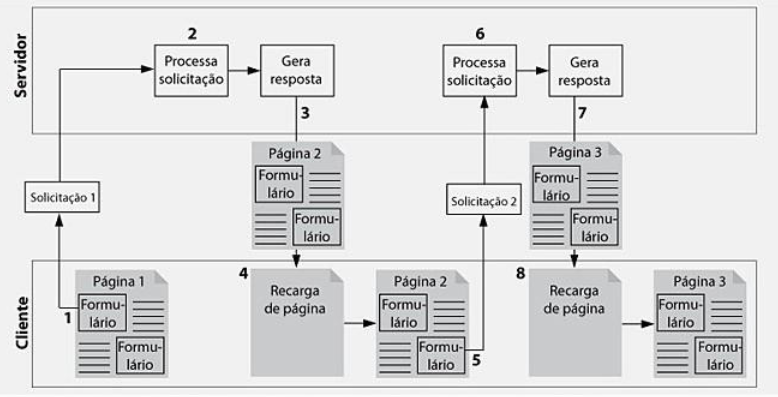
\includegraphics[width=.8\textwidth]{figuras/arquitetura_web_tradicional.png}
	 \vspace{-0.3cm}
	\\\textbf{\footnotesize Fonte: \cite{deitelAjax}}
	\label{fig:arquitetura_web_tradicional}
\end{figure}

Cada recarga na página gerava uma nova requisição ao servidor, que neste modelo é responsável por processar a requisição, gerar e enviar a resposta 
contendo a página exata que será exibida no browser do cliente. Esse delay presente nas interações com a aplicação fizeram com que os usuários 
exigissem uma forma melhor de interagir com estas aplicações. 

Para solucionar este problema de desempenho presente nas aplicações tradicionais, surgiu o Ajax. Como descrito por \cite{garrettAjax}, uma aplicação
Ajax elimina a natureza de interação Web conhecida como \textit{start-stop-start-stop} introduzindo uma camada intermediária — Ajax engine — entre 
cliente e servidor. Essa camada que permitiu à essas aplicações realizarem requisições ao servidor de forma assíncrona e atualizar parcialmente a 
página ao receber a resposta, não impedindo a interação do usuário durante o ciclo de requisição/resposta. Abaixo na Figura \ref{fig:ajax_comparison} 
podemos ver um comparativo entre aplicações web síncronas e assíncronas.

\begin{figure}[!ht]
	\centering	
	\caption[\hspace{0.1cm}Comparação aplicação web clássica e aplicação web com Ajax.]{Comparação aplicação web clássica e aplicação web com Ajax}
	  \vspace{-0.4cm}
	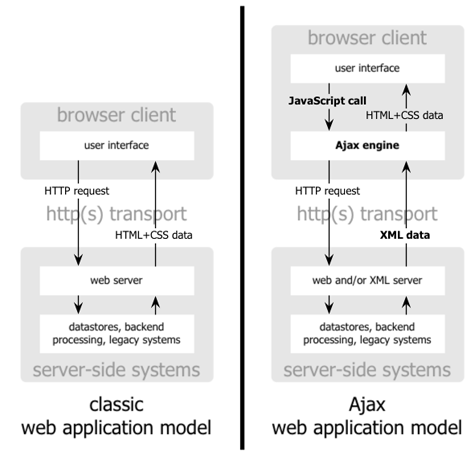
\includegraphics[width=.8\textwidth]{figuras/ajax_comparison.png}
	 \vspace{-0.3cm}
	\\\textbf{\footnotesize Fonte: \cite{garrettAjax}}
	\label{fig:ajax_comparison}
\end{figure}


Com aplicações construídas utilizando Ajax, a Web voltou à ser atrativa para usuário e tem crescido o número de aplicações web desde então. Segundo
\cite{tabulaRest} as aplicações web assumem atualmente uma importância sem precedentes em todas as áreas da sociedade. Em \cite{fieldingRest} foi apresentado o Representational State Transfer (REST) 
como um estilo arquitetural para sistemas de hipermídia distribuídos baseado no \textit{HyperText Transfer Protocol} (HTTP). Segundo 
\cite{modelingRestful}, o entendimento do REST pode ajudar na obtenção de uma melhor performace e escalabilidade, bem como diminuir o acoplamento,
como resultado aumentando a interoperabilidade, promovendo o reuso. Aplicações que seguem as restrições REST são denominadas como RESTful, estas 
aplicações consistem em um \textit{Web Service} simples que utiliza verbos HTTP para mapear ações as \textit{Create, Read, Update, Delete} (CRUD). 
Podemos ver na Tabela \ref{tab:tabela1} o mapeamento de verbos HTTP com as ações CRUD.

\begin{table}[htb]
	\centering
	\caption{\hspace{0.1cm} Relacionamento de verbos HTTP com ações CRUD}
	\vspace{-0.3cm} % espaço entre titulo e tabela
	\label{tab:tabela1}
	% Conteúdo da tabela
	\begin{tabular}{l|c}
  \hline
    \textbf{HTTP} & \textbf{Ação} \\
    \hline
      GET & Read \\
      POST & Create \\
      PUT & Update \\
      DELETE & Delete \\
     \hline
 \end{tabular}
 	\vspace{.1cm}  %espaço entre tabela e fonte
	\small
	% Fonte
	{\footnotesize\\ \textbf{Fonte: Elaborado pelo autor}}
\end{table}

Devido à este aprimoramento constante no que diz respeito ao desenvolvimento de aplicações web, a arquitetura de uma aplicação web está deixando 
de ser composta por grandes quantidades de códigos server-side, onde todo o processamento é feito no servidor, os códigos são fechados e o consumo 
de banda é maior aos proprietários do sistema, e passando a ter maior utilização de códigos client-side, onde o processamento dos scripts da página
ocorre na máquina do cliente e somente quando há necessidade de interação com o banco de dados são feitas requisições ao servidor \cite{spa01}. Neste 
contexto surgiram as \textit{Single Page Applications} (SPA) definida por \cite{spa02} aplicações compota por somente uma pagina HTML, como base para 
todas as outras páginas web da aplicação nas quais as interações feitas pelo usuário são implementadas usando JavaScript, HTML e CSS. A Figura 
\ref{fig:spa} demonstra o funcionamento de uma SPA.

\begin{figure}[!ht]
	\centering	
	\caption[\hspace{0.1cm} Ciclo de vida de uma Single Page Application.]{Ciclo de vida de uma Single Page Application}
	  \vspace{-0.4cm}
	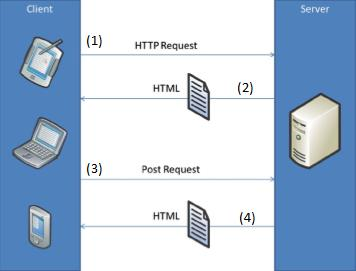
\includegraphics[width=.8\textwidth]{figuras/spa.png}
	 \vspace{-0.3cm}
	\\\textbf{\footnotesize Fonte: \cite{spa02}}
	\label{fig:spa}
\end{figure}

Em aplicações SPA, a primeira requisição realizada pelo cliente recebe como resposta uma página HTML, nesta página inicial há um extenso conteúdo de
scripts responsáveis pela navegação do usuário, sem que haja recarga da página, quando há necessidade de conteúdos presentes no servidor, esta 
comunicação é feita através de requisições AJAX, e os scripts presentes na página são responsáveis por renderizar estes conteúdos recebidos na página,
através do \textit{Document Object Model} (DOM). Toda transição de páginas neste tipo de aplicação é realizada \textit{client-side}. Uma das vantagens
da adoção deste modelo em relação ao modelo anterior é em relação ao overhead de requisições, o que torna a aplicação mais leve e permite melhor 
usabilidade para o usuário final, devido ao AJAX não bloquear a manipulação da página durante sua execução \cite{spa01}, além de facilitar a 
portabilidade da aplicação pois este modelo requer uma API \textit{server-side} bem estruturada para funcionar.